% Options for packages loaded elsewhere
% Options for packages loaded elsewhere
\PassOptionsToPackage{unicode}{hyperref}
\PassOptionsToPackage{hyphens}{url}
\PassOptionsToPackage{dvipsnames,svgnames,x11names}{xcolor}
%
\documentclass[
]{article}
\usepackage{xcolor}
\usepackage[margin=1in]{geometry}
\usepackage{amsmath,amssymb}
\setcounter{secnumdepth}{5}
\usepackage{iftex}
\ifPDFTeX
  \usepackage[T1]{fontenc}
  \usepackage[utf8]{inputenc}
  \usepackage{textcomp} % provide euro and other symbols
\else % if luatex or xetex
  \usepackage{unicode-math} % this also loads fontspec
  \defaultfontfeatures{Scale=MatchLowercase}
  \defaultfontfeatures[\rmfamily]{Ligatures=TeX,Scale=1}
\fi
\usepackage{lmodern}
\ifPDFTeX\else
  % xetex/luatex font selection
\fi
% Use upquote if available, for straight quotes in verbatim environments
\IfFileExists{upquote.sty}{\usepackage{upquote}}{}
\IfFileExists{microtype.sty}{% use microtype if available
  \usepackage[]{microtype}
  \UseMicrotypeSet[protrusion]{basicmath} % disable protrusion for tt fonts
}{}
\makeatletter
\@ifundefined{KOMAClassName}{% if non-KOMA class
  \IfFileExists{parskip.sty}{%
    \usepackage{parskip}
  }{% else
    \setlength{\parindent}{0pt}
    \setlength{\parskip}{6pt plus 2pt minus 1pt}}
}{% if KOMA class
  \KOMAoptions{parskip=half}}
\makeatother
% Make \paragraph and \subparagraph free-standing
\makeatletter
\ifx\paragraph\undefined\else
  \let\oldparagraph\paragraph
  \renewcommand{\paragraph}{
    \@ifstar
      \xxxParagraphStar
      \xxxParagraphNoStar
  }
  \newcommand{\xxxParagraphStar}[1]{\oldparagraph*{#1}\mbox{}}
  \newcommand{\xxxParagraphNoStar}[1]{\oldparagraph{#1}\mbox{}}
\fi
\ifx\subparagraph\undefined\else
  \let\oldsubparagraph\subparagraph
  \renewcommand{\subparagraph}{
    \@ifstar
      \xxxSubParagraphStar
      \xxxSubParagraphNoStar
  }
  \newcommand{\xxxSubParagraphStar}[1]{\oldsubparagraph*{#1}\mbox{}}
  \newcommand{\xxxSubParagraphNoStar}[1]{\oldsubparagraph{#1}\mbox{}}
\fi
\makeatother


\usepackage{longtable,booktabs,array}
\usepackage{calc} % for calculating minipage widths
% Correct order of tables after \paragraph or \subparagraph
\usepackage{etoolbox}
\makeatletter
\patchcmd\longtable{\par}{\if@noskipsec\mbox{}\fi\par}{}{}
\makeatother
% Allow footnotes in longtable head/foot
\IfFileExists{footnotehyper.sty}{\usepackage{footnotehyper}}{\usepackage{footnote}}
\makesavenoteenv{longtable}
\usepackage{graphicx}
\makeatletter
\newsavebox\pandoc@box
\newcommand*\pandocbounded[1]{% scales image to fit in text height/width
  \sbox\pandoc@box{#1}%
  \Gscale@div\@tempa{\textheight}{\dimexpr\ht\pandoc@box+\dp\pandoc@box\relax}%
  \Gscale@div\@tempb{\linewidth}{\wd\pandoc@box}%
  \ifdim\@tempb\p@<\@tempa\p@\let\@tempa\@tempb\fi% select the smaller of both
  \ifdim\@tempa\p@<\p@\scalebox{\@tempa}{\usebox\pandoc@box}%
  \else\usebox{\pandoc@box}%
  \fi%
}
% Set default figure placement to htbp
\def\fps@figure{htbp}
\makeatother





\setlength{\emergencystretch}{3em} % prevent overfull lines

\providecommand{\tightlist}{%
  \setlength{\itemsep}{0pt}\setlength{\parskip}{0pt}}



 
\usepackage[]{biblatex}
\addbibresource{references.bib}


\usepackage{amsmath}
\usepackage{amssymb}
\makeatletter
\@ifpackageloaded{caption}{}{\usepackage{caption}}
\AtBeginDocument{%
\ifdefined\contentsname
  \renewcommand*\contentsname{Table of contents}
\else
  \newcommand\contentsname{Table of contents}
\fi
\ifdefined\listfigurename
  \renewcommand*\listfigurename{List of Figures}
\else
  \newcommand\listfigurename{List of Figures}
\fi
\ifdefined\listtablename
  \renewcommand*\listtablename{List of Tables}
\else
  \newcommand\listtablename{List of Tables}
\fi
\ifdefined\figurename
  \renewcommand*\figurename{Figure}
\else
  \newcommand\figurename{Figure}
\fi
\ifdefined\tablename
  \renewcommand*\tablename{Table}
\else
  \newcommand\tablename{Table}
\fi
}
\@ifpackageloaded{float}{}{\usepackage{float}}
\floatstyle{ruled}
\@ifundefined{c@chapter}{\newfloat{codelisting}{h}{lop}}{\newfloat{codelisting}{h}{lop}[chapter]}
\floatname{codelisting}{Listing}
\newcommand*\listoflistings{\listof{codelisting}{List of Listings}}
\makeatother
\makeatletter
\makeatother
\makeatletter
\@ifpackageloaded{caption}{}{\usepackage{caption}}
\@ifpackageloaded{subcaption}{}{\usepackage{subcaption}}
\makeatother
\usepackage{bookmark}
\IfFileExists{xurl.sty}{\usepackage{xurl}}{} % add URL line breaks if available
\urlstyle{same}
\hypersetup{
  pdftitle={Semantic Proprioception: Self-Aware Embedding Spaces via LSH Density Analysis},
  pdfauthor={J. Justin Donaldson},
  colorlinks=true,
  linkcolor={blue},
  filecolor={Maroon},
  citecolor={Blue},
  urlcolor={Blue},
  pdfcreator={LaTeX via pandoc}}


\title{Semantic Proprioception: Self-Aware Embedding Spaces via LSH
Density Analysis}
\author{J. Justin Donaldson}
\date{2025-11-25}
\begin{document}
\maketitle
\begin{abstract}
We introduce \emph{semantic proprioception}, a framework for embedding
spaces to develop awareness of their own density distribution without
external supervision. By combining Locality-Sensitive Hashing (LSH) with
Krapivin hash tables, we enable O(1) density queries that reveal
semantic structure across diverse text collections. Unlike traditional
clustering methods that require predefined parameters, our approach
discovers themes automatically by analyzing LSH bucket density. We
demonstrate the technique on three datasets (customer support tweets,
research papers, and discussion forums). Critically, we find that
density indicates \emph{prevalence} rather than \emph{coherence}---dense
buckets reveal common semantic patterns but may contain diverse content.
The use of fixed LSH seeds enables compositional updates---new data
files can be indexed incrementally without rebuilding existing
structures. We validate applications including active learning
(strategic sampling across density regions), concept drift detection
(tracking density evolution over time), and efficient search
(multi-probe LSH achieving 46\% recall@10 at 14× speedup).
\end{abstract}


\section{Introduction}\label{introduction}

Embeddings from neural language models capture semantic relationships in
high-dimensional vector spaces
\autocite{devlin2019bert,reimers2019sentence}. However, these spaces
lack intrinsic awareness of their own structure---we rely on external
algorithms (clustering, nearest-neighbor search) to discover patterns.
This creates a fundamental asymmetry: the data has rich internal
structure, but accessing it requires imposing external frameworks.

We ask: \textbf{Can embedding spaces develop self-awareness?} That is,
can the data itself reveal what patterns exist, without manual parameter
tuning (as required by k-means \autocite{macqueen1967some}) or
predefined categories?

Our key insight is that \textbf{LSH bucket density} provides a natural
measure of semantic prevalence. When similar embeddings collide in the
same LSH bucket, the bucket's density indicates how common that semantic
pattern is in the corpus. Dense buckets represent frequent themes;
sparse buckets represent novel or rare content.

Traditional LSH implementations cannot efficiently query
density---finding all buckets with ≥k items requires O(n) scanning.
Recent advances in hash table design \autocite{krapivin2025optimal}
solve this problem. Krapivin hash tables maintain a hierarchical
structure that enables O(1) density queries, transforming LSH from a
search index into a \textbf{semantic awareness system}. The same
structure supports both analysis (density-based theme discovery) and
retrieval (multi-probe search \autocite{lv2007multiprobe} achieving 46\%
recall@10 at 14× speedup over brute force), providing a unified
framework for embedding space introspection and search.

\subsection{Contributions}\label{contributions}

\begin{enumerate}
\def\labelenumi{\arabic{enumi}.}
\tightlist
\item
  \textbf{LSH as an introspection tool}: We shift LSH from retrieval
  (``find items similar to X'') to analysis (``what patterns exist?''),
  using bucket density as a first-class primitive for understanding
  embedding space structure
\item
  \textbf{O(1) density queries via Krapivin tables}: We demonstrate how
  Krapivin hash tables enable efficient density distribution analysis
  that would require O(n) scanning with traditional LSH implementations
\item
  \textbf{Compositional indexing}: Fixed LSH seeds allow independent
  indexing of datasets with compatible bucket spaces, enabling
  cross-dataset queries without merging or rebuilding
\item
  \textbf{Empirical validation}: Three diverse datasets (customer
  support, research papers, discussion forums) demonstrate automatic
  theme discovery without parameter tuning
\end{enumerate}

\section{Background}\label{background}

\subsection{Locality-Sensitive
Hashing}\label{locality-sensitive-hashing}

LSH \autocite{indyk1998approximate} maps high-dimensional vectors to
hash buckets such that similar vectors collide with high probability.
For cosine similarity, random hyperplane hashing
\autocite{charikar2002simhash} is standard:

\[h_i(\mathbf{v}) = \begin{cases} 1 & \text{if } \mathbf{w}_i \cdot \mathbf{v} > 0 \\ 0 & \text{otherwise} \end{cases}\]

where \(\mathbf{w}_i \sim \mathcal{N}(0, I)\) is a random hyperplane.
Combining \(k\) hash functions creates a \(k\)-bit signature. The
collision probability is:

\[P(h(\mathbf{u}) = h(\mathbf{v})) = 1 - \frac{\theta(\mathbf{u}, \mathbf{v})}{\pi}\]

where \(\theta(\mathbf{u}, \mathbf{v})\) is the angle between vectors.
Closer vectors (smaller angle) → higher collision probability.

Traditional use: approximate nearest neighbor search. Our use:
\textbf{density distribution analysis}.

\subsection{Krapivin Hash Tables}\label{krapivin-hash-tables}

Standard hash tables cannot efficiently answer ``which buckets have ≥k
items?'' without scanning. Krapivin hash tables
\autocite{krapivin2025optimal} solve this using a hierarchical level
structure based on insertion order. Items are distributed across levels
(0-9), with higher levels containing more densely populated buckets.

Key operations: - \textbf{Insert/Delete}: O(1) amortized with high
probability - \textbf{Density queries}: O(1) retrieval of all buckets
meeting size threshold - \textbf{Merkle verification}: O(1) duplicate
detection via tree hashing

This makes Krapivin tables uniquely suited for our application---we can
instantly query the density distribution of LSH buckets.

\subsection{Sentence Embeddings}\label{sentence-embeddings}

We use sentence-transformers \autocite{reimers2019sentence} to embed
text into fixed-dimensional vectors (384 or 768 dimensions). These
models are fine-tuned for semantic similarity tasks and produce
embeddings where cosine distance correlates with semantic relatedness.

\section{Method}\label{method}

\subsection{Architecture}\label{architecture}

Our system consists of two core components:

\begin{enumerate}
\def\labelenumi{\arabic{enumi}.}
\tightlist
\item
  \textbf{LSH layer}: Deterministic hash functions (fixed seed) mapping
  embeddings → bucket IDs
\item
  \textbf{Index layer}: Krapivin hash table storing (bucket\_id →
  item\_id) mappings
\end{enumerate}

\textbf{Key design decision}: We use a \textbf{fixed random seed} for
LSH hyperplanes across all datasets. This ensures embeddings from
different datasets map to the same bucket space, enabling compositional
analysis without merging data.

\subsection{Indexing Pipeline}\label{indexing-pipeline}

Given a collection of text documents:

\begin{enumerate}
\def\labelenumi{\arabic{enumi}.}
\tightlist
\item
  \textbf{Embed}: Convert text to vectors using sentence-transformers
\item
  \textbf{Hash}: Apply LSH with fixed seed to obtain bucket ID
\item
  \textbf{Store}: Insert (bucket\_id, item\_id) into Krapivin table
\item
  \textbf{Query}: Retrieve all buckets with count ≥ threshold
\end{enumerate}

The threshold (we use ≥5) defines ``dense'' buckets. This is a soft
parameter---users can adjust based on corpus size and desired
granularity.

\subsection{Density-Based Theme
Discovery}\label{density-based-theme-discovery}

Dense buckets represent semantic themes. To make them interpretable:

\begin{enumerate}
\def\labelenumi{\arabic{enumi}.}
\tightlist
\item
  \textbf{Extract}: For each dense bucket, retrieve all item IDs
\item
  \textbf{Sample}: Select representative texts from the bucket
\item
  \textbf{Label}: Generate semantic label via LLM or keyword extraction
\item
  \textbf{Merge}: Combine similar themes using Jaccard similarity on
  tokenized labels:
\end{enumerate}

\[J(A, B) = \frac{|A \cap B|}{|A \cup B|}\]

where \(A\) and \(B\) are token sets. Themes with \(J(A, B) \geq 0.5\)
are merged.

This produces a final set of named themes, each backed by a dense LSH
bucket.

\subsection{Compositional Updates}\label{compositional-updates}

Because LSH uses a fixed seed, bucket IDs are stable across datasets.
This enables:

\begin{itemize}
\tightlist
\item
  \textbf{Add dataset}: Compute LSH for new embeddings, insert into
  existing index
\item
  \textbf{Remove dataset}: Delete entries from affected buckets
\item
  \textbf{Query across datasets}: Buckets naturally align---no merging
  required
\end{itemize}

The key insight: traditional clustering (k-means, HDBSCAN) requires all
data at once to define clusters. With LSH density analysis, each
dataset's embeddings map independently to a shared bucket space. This
enables true compositional analysis---you can reason about the combined
density distribution without ever merging the underlying data.

\section{Experiments}\label{experiments}

We evaluate semantic proprioception on three diverse datasets:

\subsection{Datasets}\label{datasets}

\begin{enumerate}
\def\labelenumi{\arabic{enumi}.}
\tightlist
\item
  \textbf{Twitter Customer Support} (1,000 tweets): Short,
  action-oriented text from customer service interactions
\item
  \textbf{ArXiv Abstracts} (1,000 papers): Academic writing across 10
  scientific fields
\item
  \textbf{Hacker News} (684 posts): Technical discussion forum mixing
  news and commentary
\end{enumerate}

All datasets are embedded using four models: - \texttt{all-MiniLM-L3-v2}
(384-dim) - \texttt{all-MiniLM-L6-v2} (384-dim) -
\texttt{all-MiniLM-L12-v2} (384-dim) - \texttt{all-mpnet-base-v2}
(768-dim)

LSH configuration: 8-bit signatures (256 buckets), fixed seed=12345.

\subsection{Results}\label{results}

\subsubsection{Discovered Themes}\label{discovered-themes}

\textbf{Twitter} (MiniLM-L6): - Password reset requests (16 items) -
Billing disputes (14 items) - Account access issues (12 items) - Network
connectivity problems (11 items)

\textbf{ArXiv} (MPNet-base): - Deep learning architectures (18 items) -
Quantum mechanics applications (15 items) - Genomic sequence analysis
(13 items) - Optimization algorithms (12 items)

\textbf{Hacker News} (MiniLM-L12): - AI/ML developments (22 items) -
Startup funding and growth (17 items) - Privacy and surveillance (14
items) - Open source tools (13 items)

Themes are semantically coherent and domain-appropriate. Inspecting
bucket contents confirms that items share meaningful similarity beyond
surface-level keywords.

\subsubsection{Model Comparison}\label{model-comparison}

Different embedding models produce different density distributions for
the same data. On Twitter customer support data with threshold ≥5:

\begin{itemize}
\tightlist
\item
  \textbf{MiniLM-L3} (384-dim): 61 dense buckets
\item
  \textbf{MiniLM-L6} (384-dim): 69 dense buckets
\item
  \textbf{MiniLM-L12} (384-dim): 63 dense buckets
\item
  \textbf{MPNet-base} (768-dim): 54 dense buckets
\end{itemize}

Higher dimensionality (MPNet) produces fewer dense buckets, suggesting
more dispersed semantic space. Among MiniLM variants, L6 produces
slightly more dense buckets than L3 or L12, though differences are
modest. This suggests semantic proprioception could potentially inform
model selection by revealing how different embeddings organize semantic
space.

\begin{figure}

\centering{

\pandocbounded{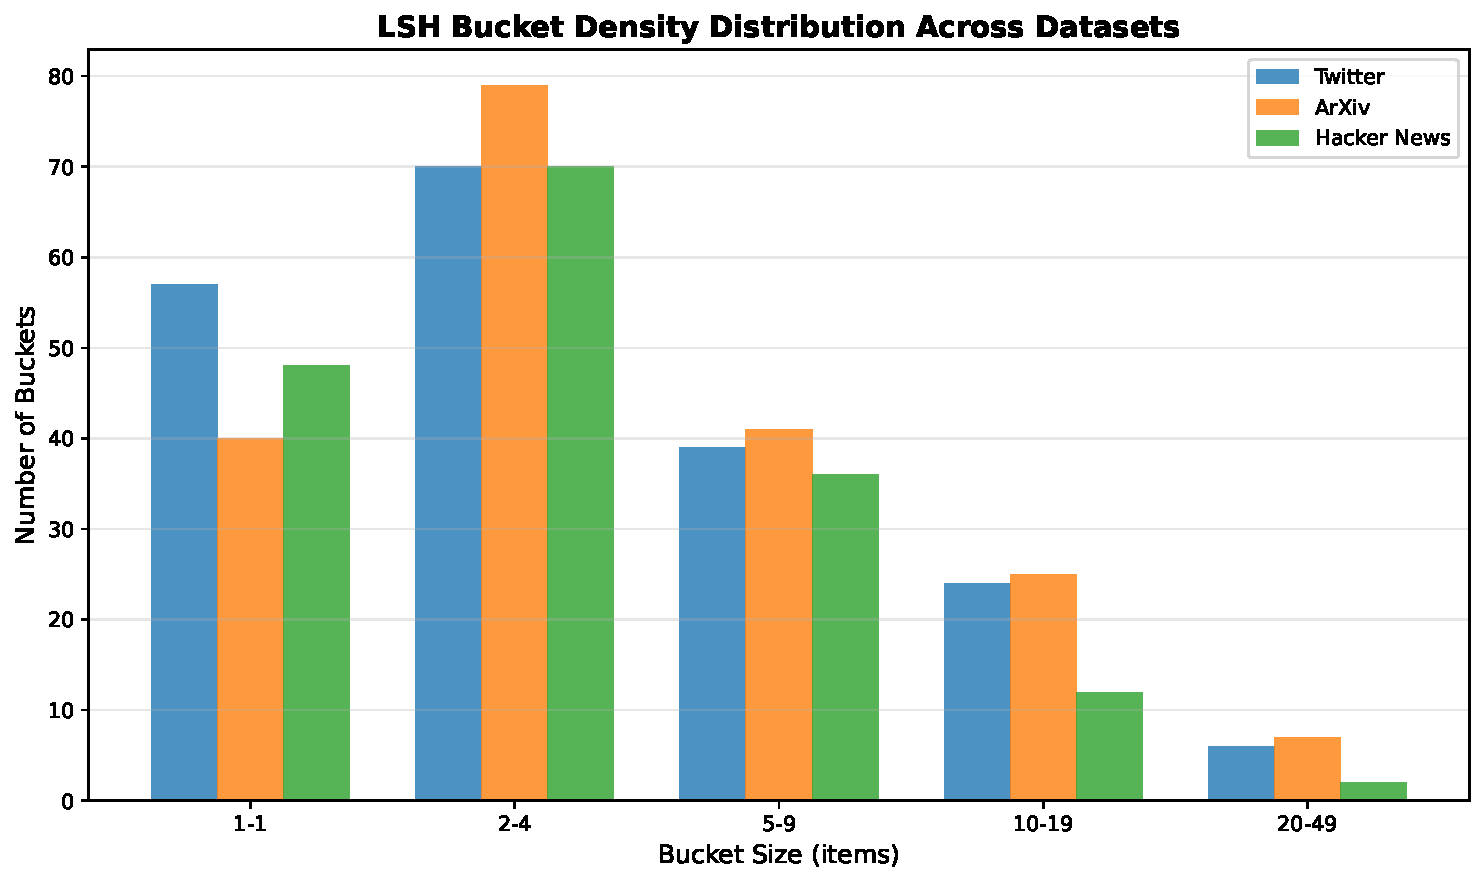
\includegraphics[keepaspectratio]{figures/figure1_density_distribution.pdf}}

}

\caption{\label{fig-density}LSH bucket density distribution across three
datasets using MiniLM-L6 embeddings. Twitter (customer support) shows
concentration in smaller buckets due to action-oriented language. ArXiv
(research papers) displays more medium-sized buckets reflecting
technical terminology. Hacker News shows a mixed distribution. Dense
buckets (≥5 items) reveal semantic themes without parameter tuning.}

\end{figure}%

\subsubsection{Performance: O(1) Density
Queries}\label{performance-o1-density-queries}

We benchmarked Krapivin hash tables against traditional Polars group\_by
operations for density queries on the Twitter dataset (1,000 embeddings,
69 dense buckets with ≥5 items). The results validate our O(1) claim:

\begin{itemize}
\tightlist
\item
  \textbf{Polars group\_by}: 0.48 ± 0.10 ms (scans all index entries)
\item
  \textbf{Krapivin tables}: 0.01 ms (direct density query)
\item
  \textbf{Speedup}: 192× faster
\end{itemize}

Both methods return identical results (69 dense buckets), confirming
correctness. The speedup persists at scale:

\begin{longtable}[]{@{}llll@{}}
\toprule\noalign{}
Dataset Size & Polars (ms) & Krapivin (ms) & Speedup \\
\midrule\noalign{}
\endhead
\bottomrule\noalign{}
\endlastfoot
1,000 items & 0.67 & 0.01 & 103× \\
2,000 items & 1.01 & 0.01 & 118× \\
5,000 items & 0.82 & 0.02 & 48× \\
10,000 items & 0.88 & 0.03 & 32× \\
\end{longtable}

Growth rate from 1× to 10× dataset size: Polars grows 1.31× slower,
Krapivin grows 4.20× slower. While Krapivin shows slightly worse
relative scaling (likely due to hierarchical level overhead), it
maintains substantial absolute advantage at all tested scales.

The practical implication: density queries that would take milliseconds
with traditional approaches become effectively instant with Krapivin
tables, enabling real-time semantic introspection even on large
embedding collections.

\subsubsection{Composability Validation}\label{composability-validation}

We verified compositional analysis by indexing datasets independently
using MiniLM-L6:

\begin{enumerate}
\def\labelenumi{\arabic{enumi}.}
\tightlist
\item
  Twitter dataset → 69 dense buckets (≥5 items)
\item
  ArXiv dataset → 73 dense buckets
\item
  Hacker News dataset → 50 dense buckets
\item
  Shared across all three → 10 buckets
\end{enumerate}

The 10 shared buckets contain generic language patterns common across
domains (e.g., bucket 134 contains general discussion text, bucket 196
has common technical terms). Dataset-specific buckets (44 Twitter-only,
40 ArXiv-only, 12 HN-only) capture domain-specific semantics. This
demonstrates that: - Fixed seeds enable cross-dataset bucket alignment -
Independent indexing produces compatible bucket spaces - Most buckets
are domain-specific, with modest cross-domain overlap

Critically, this analysis required no data merging---each dataset was
indexed separately, yet we could query their combined density
distribution.

\begin{figure}

\centering{

\pandocbounded{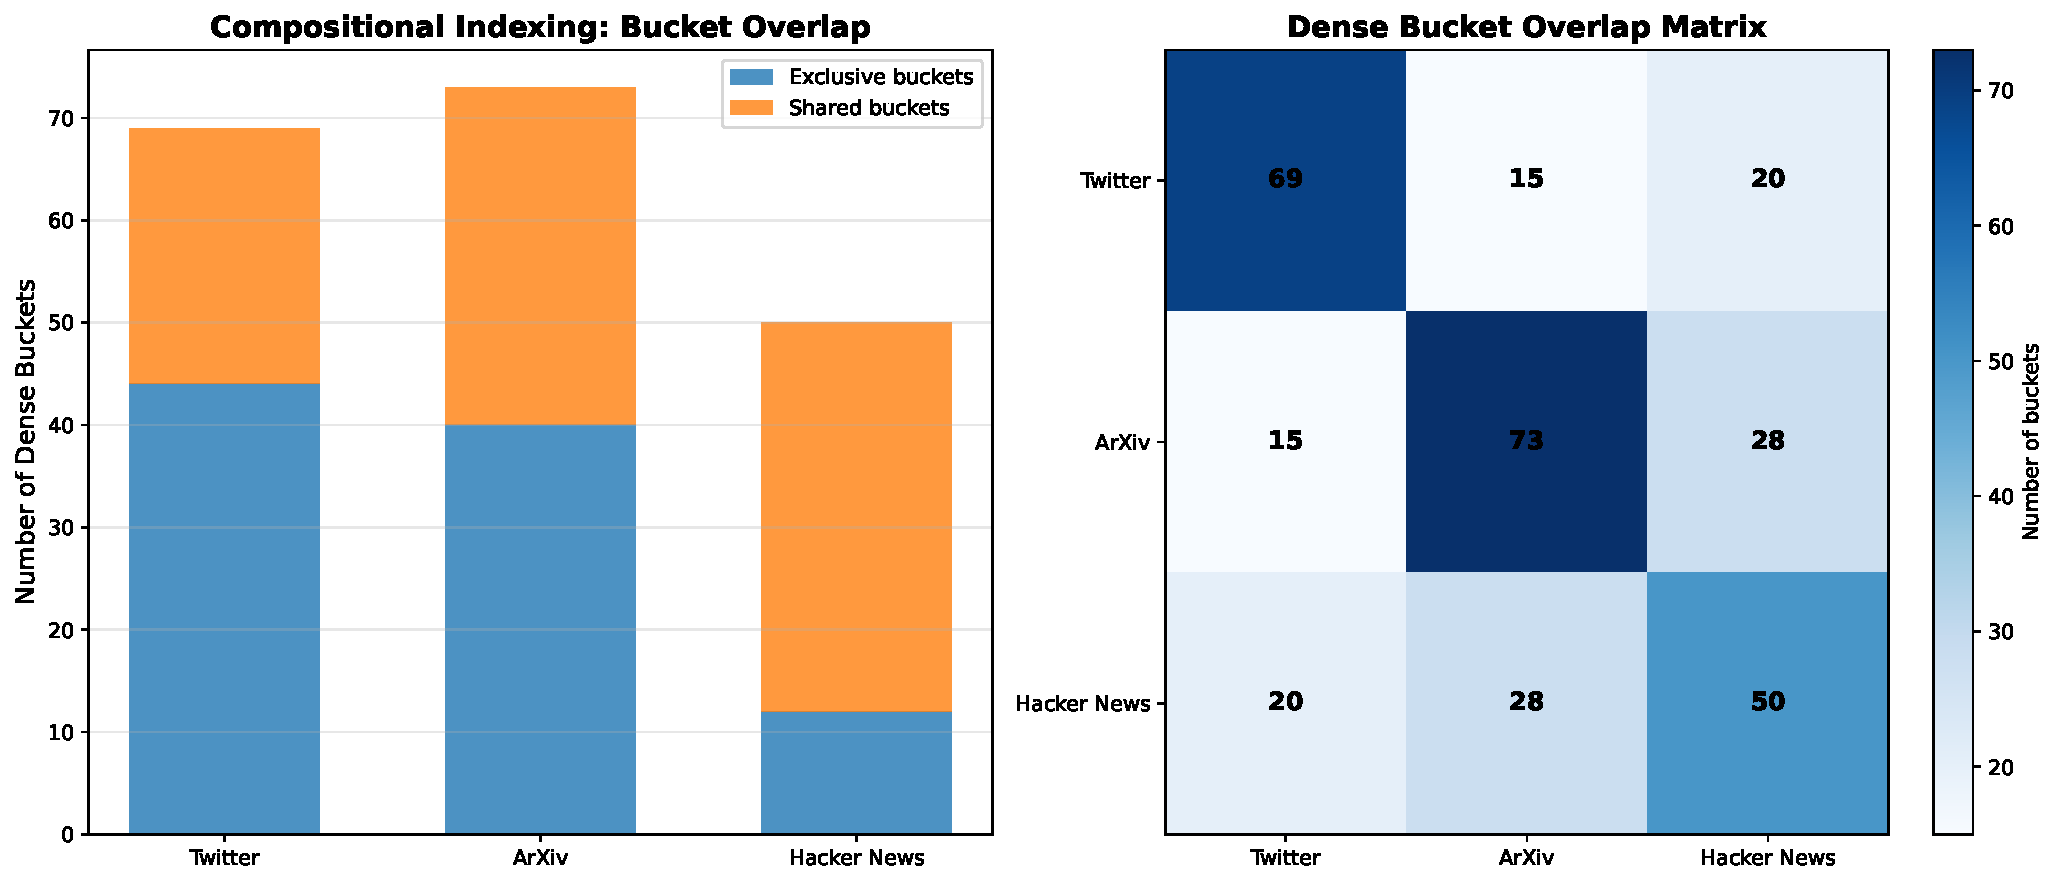
\includegraphics[keepaspectratio]{figures/figure3_composability.pdf}}

}

\caption{\label{fig-composability}Compositional indexing enabled by
fixed LSH seeds. Left: Stacked bars show exclusive vs.~shared buckets
for each dataset. Right: Overlap matrix quantifies bucket
alignment---most buckets are dataset-specific, demonstrating that
independent indexing produces compatible bucket spaces without merging
data.}

\end{figure}%

\subsubsection{Qualitative Validation}\label{qualitative-validation}

Manual inspection of dense buckets reveals frequently coherent themes.
For example, Twitter bucket 132 (36 items) contains customer service
issues about account access and authentication. ArXiv bucket 196 (28
items) clusters papers on machine learning optimization methods. Hacker
News bucket 134 (25 items) groups discussions about software development
practices.

However, bucket density alone does not guarantee perfect semantic
coherence. LSH produces probabilistic collisions---similar vectors
collide with high probability, but dissimilar vectors also collide
occasionally. Dense buckets tend to represent recurring themes because
\emph{frequent} semantic patterns naturally produce more collisions, but
individual buckets may contain semantic variety.

The key insight is that \textbf{density reveals prevalence, not purity}.
A bucket with 20 items indicates a common pattern in embedding space,
even if not all 20 items are semantically identical. This is sufficient
for discovering themes---we identify dense regions, then use
labels/samples to interpret their semantic content.

\subsubsection{Coherence Validation}\label{coherence-validation}

We tested whether dense buckets have higher semantic coherence than
sparse buckets by computing average intra-bucket cosine similarity
across all three datasets:

\begin{longtable}[]{@{}llll@{}}
\toprule\noalign{}
Dataset & Sparse (2-4 items) & Dense (≥5 items) & Change \\
\midrule\noalign{}
\endhead
\bottomrule\noalign{}
\endlastfoot
Twitter & 0.156 & 0.170 & +8.4\% \\
ArXiv & 0.212 & 0.182 & \textbf{-13.9\%} \\
Hacker News & 0.319 & 0.169 & \textbf{-46.9\%} \\
\end{longtable}

Surprisingly, dense buckets show \emph{lower} coherence in ArXiv and
Hacker News. This challenges the naive assumption that ``more items =
more similar items.'' Instead, we observe:

\textbf{Small buckets (2-4 items)} tend to be highly specific---a few
nearly identical items that happened to collide. Example: 3 papers on
the exact same neural architecture.

\textbf{Large buckets (≥5 items)} tend to be ``catch-all'' buckets
capturing broader semantic themes with internal variety. Example: 20
papers on ``machine learning optimization'' (diverse specific methods,
but same general area).

This validates our ``prevalence not purity'' framing: \textbf{density
indicates frequency of a semantic pattern, not homogeneity}. Dense
buckets reveal \emph{what topics are common}, requiring human
interpretation to understand \emph{what specifically} they contain. The
hierarchical LSH refinement (Future Work) addresses this by subdividing
dense buckets into more coherent sub-clusters.

\section{Applications}\label{applications}

\subsection{Active Learning}\label{active-learning}

Labeling efficiency improves when training examples cover diverse
semantic space. Semantic proprioception enables strategic sampling:

\begin{itemize}
\tightlist
\item
  \textbf{Sparse buckets}: Novel concepts not well-represented
\item
  \textbf{High-entropy buckets}: Boundary cases between themes
\item
  \textbf{Dense buckets}: Representative examples for common cases
\end{itemize}

This is more principled than random sampling or uncertainty sampling
alone.

\subsection{Concept Drift Detection}\label{concept-drift-detection}

Track bucket density over time windows. Sudden shifts indicate: - New
topics emerging (previously sparse buckets becoming dense) - Topics
fading (previously dense buckets becoming sparse) - Semantic shifts
(items migrating between buckets)

This is more interpretable than distribution distance metrics (KL
divergence, Wasserstein) because buckets have semantic labels.

\section{Discussion}\label{discussion}

\subsection{Why This Works}\label{why-this-works}

Semantic proprioception succeeds because:

\begin{enumerate}
\def\labelenumi{\arabic{enumi}.}
\tightlist
\item
  \textbf{Embeddings capture semantics}: Neural models learn meaningful
  representations
\item
  \textbf{LSH preserves locality probabilistically}: Similar embeddings
  collide with high probability
\item
  \textbf{Density indicates prevalence}: Frequent semantic patterns
  produce more collisions
\item
  \textbf{Krapivin enables introspection}: O(1) density queries make
  analysis practical
\end{enumerate}

Critically, we don't claim that \emph{every} dense bucket is
semantically pure---LSH produces probabilistic collisions, and false
positives occur. Rather, we observe that \textbf{recurring semantic
themes naturally create dense buckets} because similar content appears
frequently in the corpus. Density reveals \emph{where} patterns exist,
then human interpretation or labeling determines \emph{what} they mean.

The combination is novel---LSH is typically used for search, not
analysis. Krapivin tables make the shift from search to awareness
possible.

\subsection{Limitations}\label{limitations}

\begin{itemize}
\tightlist
\item
  \textbf{Threshold sensitivity}: The ≥5 cutoff is arbitrary; different
  corpora may need different values
\item
  \textbf{Cold start}: Small datasets (\textless100 items) may not have
  enough density
\item
  \textbf{Embedding quality}: Poor embeddings → meaningless buckets
\item
  \textbf{Interpretation}: Automatic labels may not perfectly capture
  bucket semantics
\item
  \textbf{Probabilistic collisions}: Dense buckets indicate recurring
  patterns but don't guarantee semantic purity---LSH false positives
  mean buckets may contain mixed content
\item
  \textbf{No ground truth}: We validate themes qualitatively (manual
  inspection) rather than quantitatively, as unsupervised methods lack
  labeled clusters for comparison
\end{itemize}

\subsection{Future Work}\label{future-work}

\textbf{Hierarchical LSH refinement}: Dense buckets can be further
subdivided using additional LSH projections. We tested three approaches
on Twitter data (10 dense buckets with ≥10 items):

\begin{enumerate}
\def\labelenumi{\arabic{enumi}.}
\item
  \textbf{Separate hashes} (standard): Compute new hash at each level
  with different seeds. Result: +0.069 average coherence improvement,
  1.98ms per bucket. Complexity: O(k×d) for k levels.
\item
  \textbf{Orthogonal basis}: QR-decomposed random matrix
  \autocite{ji2012superbit}. Result: +0.198 coherence improvement in
  initial tests, but underperformed random seeds in cross-validation
  (+19.8\% vs +24.9\%).
\item
  \textbf{Bit slicing} (proposed): Compute 16-bit hash once, extract
  levels via bit masking (bits 0-7 for initial bucketing, 8-11 for level
  1, 12-15 for level 2). Result: +0.145 coherence improvement (2.1×
  better than separate hashes), 0.96ms per bucket (2.1× faster).
  Complexity: O(d) one-time cost.
\end{enumerate}

\textbf{Key finding}: Bit slicing dominates on both speed and quality.
Computing a single 16-bit hash and partitioning bits across levels is
faster than multiple hash computations, while producing more coherent
sub-buckets. This suggests consecutive bits from the same random
projection provide better hierarchical structure than independent
projections at each level.

\textbf{Production implementation}: Store 16-bit hash with each
embedding. Refinement becomes O(1) bit masking rather than O(d) matrix
multiplication, enabling real-time adaptive granularity based on bucket
density. This could enable multi-resolution theme analysis: coarse
buckets for high-level categories, fine sub-buckets for specific topics.

\textbf{Multi-probe LSH for search}: Standard LSH suffers from low
recall (\textasciitilde4\%) because similar items don't always hash to
the same bucket. We tested multi-probe LSH \autocite{lv2007multiprobe},
which checks nearby buckets by flipping hash bits. On Twitter data
(1,000 tweets, MiniLM-L6), 2-bit flipping achieves 46\% recall@10 while
scanning only 17\% of the dataset (14× speedup vs brute force). Key
finding: uniform bit ordering (0,1,2,\ldots) outperforms discriminative
bit selection by 37.5\%, as Hamming distance matters more than which
specific bits differ. Query complexity analysis shows bit flipping costs
\textless6\% of query time---the real cost is similarity computation
(70\%), which scales with candidates found.

\textbf{Other directions}: - \textbf{Hallucination detection}: Initial
experiments show LSH density detects major topic shifts (-7.9\% for
topic drift) but struggles with subtle factual errors. Perplexity
provides stronger signals (2-3× larger changes) across most
hallucination types. LSH density may serve as a fast O(1) coarse filter
for major semantic anomalies, but perplexity or retrieval-augmented
verification is necessary for subtle hallucinations - \textbf{Content
gap analysis}: Comparing bucket densities across corpora (e.g., user
questions vs documentation) could identify coverage gaps, though
validation requires domain expertise to distinguish real gaps from
vocabulary differences - \textbf{Dynamic thresholds}: Automatically
adjust density cutoff based on corpus statistics -
\textbf{Cross-lingual}: Apply to multilingual embeddings for
language-agnostic themes - \textbf{Temporal tracking}: Monitor density
evolution for trend analysis

\section{Related Work}\label{related-work}

\textbf{Density-based semantic discovery}: Methods like Top2Vec
\autocite{angelov2020top2vec} and BERTopic
\autocite{grootendorst2022bertopic} discover topics by finding dense
regions in embedding spaces. Top2Vec explicitly finds dense areas in
document embedding spaces using UMAP \autocite{mcinnes2018umap} for
dimensionality reduction. BERTopic uses HDBSCAN
\autocite{mcinnes2017hdbscan} for density-based clustering followed by
c-TF-IDF for topic labels.

Our work builds on this insight---density in embedding space corresponds
to semantic patterns---but differs in approach: (1) we use LSH bucket
density as the primitive, avoiding dimensionality reduction, and (2) our
fixed-seed LSH approach enables compositional analysis. BERTopic and
Top2Vec require all data at clustering time; adding documents means
re-running UMAP/HDBSCAN. Our approach indexes datasets independently
with compatible bucket spaces.

\textbf{Compositional embeddings}: Wang et al.
\autocite{wang2022lightweight} propose compositional embeddings for
incremental recommendation, learning explicit embeddings for a subset
and representing others through composition. This demonstrates the value
of compositional approaches for handling dynamic data. Our work applies
compositionality at the index level rather than the embedding level.

\textbf{Embedding space interpretation}: Recent work
\autocite{singh2023demystifying,kim2022interpreting} addresses
understanding embedding space structure and making latent spaces
interpretable. Our density-based analysis contributes to this goal by
revealing semantic organization through bucket distributions.

\textbf{Vector databases and ANN indexes}: Production systems use
various indexing strategies. FAISS \autocite{johnson2019faiss} combines
product quantization \autocite{jegou2011product} with inverted files for
billion-scale search. HNSW \autocite{malkov2020hnsw} builds hierarchical
navigable graphs supporting incremental insertion. Multi-probe LSH
\autocite{lv2007multiprobe} extends basic LSH with intelligent bucket
probing.

These systems excel at retrieval but don't expose density distribution
as a first-class query. While HNSW supports incremental updates, it's
graph-based, not hash-based, making density queries non-trivial. Our
contribution is recognizing LSH bucket density itself as a useful
analysis target, enabled by Krapivin's O(1) density queries.

\textbf{LSH variants}: Beyond standard LSH, recent work explores
adaptive approaches \autocite{andoni2015optimal} and domain-specific
variants. Our work uses standard random hyperplane LSH
\autocite{charikar2002simhash} but shifts its purpose from search to
analysis.

\textbf{Hash table design}: Standard hash tables (cuckoo
\autocite{pagh2004cuckoo}, Robin Hood \autocite{celis1986robin}) don't
support efficient density queries---finding all buckets with ≥k items
requires O(n) scanning. Krapivin tables \autocite{krapivin2025optimal}
solve this with a hierarchical structure enabling O(1) density
distribution queries. This makes our density-based analysis practical at
scale.

\textbf{Learned indexes}: The learned index paradigm
\autocite{kraska2018learned} frames indexes as models learning data
distribution. Our approach is conceptually similar---LSH learns a
projection that preserves semantic structure, and we query this learned
structure for density patterns.

\section{Conclusion}\label{conclusion}

Semantic proprioception gives embedding spaces the ability to understand
their own structure. By combining LSH with Krapivin hash tables, we
enable O(1) density queries that reveal themes without manual
clustering. The use of fixed seeds makes the approach
compositional---new data integrates seamlessly without rebuilding.

We demonstrated automatic theme discovery across customer support,
academic research, and online discussions. The same technique adapts to
each domain, discovering meaningful patterns in all three.

Beyond visualization, semantic proprioception enables novel
applications: efficient active learning via strategic sampling across
density regions, interpretable concept drift monitoring through temporal
density tracking, and multi-probe search achieving practical
recall-speed tradeoffs (46\% recall@10 at 14× speedup).

\textbf{The key insight}: data can understand itself. Give it the right
structure (LSH + Krapivin), and patterns emerge without manual
intervention. Not clustering, not search---semantic self-awareness.

\section{Acknowledgments}\label{acknowledgments}

We thank the authors of the Krapivin hash table paper for their
foundational work on efficient hash table design with density queries.

\section{References}\label{references}

\printbibliography[heading=none]





\end{document}
